\input{../preamble.tex}

\lecturenumber{14}
\title{Memory}
\version{1.0.0}

\usetikzlibrary{intersections} % /tikz/name path

\tikzset{swapin/.style args = {(#1,#2)}{%
    row #1 column #2/.style={nodes={text=red}}}}

\begin{document}

\begin{frame}[plain, noframenumbering]
    \titlepage
\end{frame}

\begin{slide}

    \slidetitle{Using the Page Tables for Every Memory Access is Slow}

    We need to follow pointers across multiple levels of page tables!
    \medskip

    We'll likely access the same page multiple times
    
    (close to the first access time)
    \medskip

    A process may only need a few VPN $\rightarrow$ PPN mappings at a time
    \medskip

    Our solution is another computer science classic: caching

\end{slide}

\begin{slide}

    \slidetitle{A Translation Look-Aside Buffer (TLB) Caches PTEs}
	
	\vspace{-5mm}
	
    \centering
    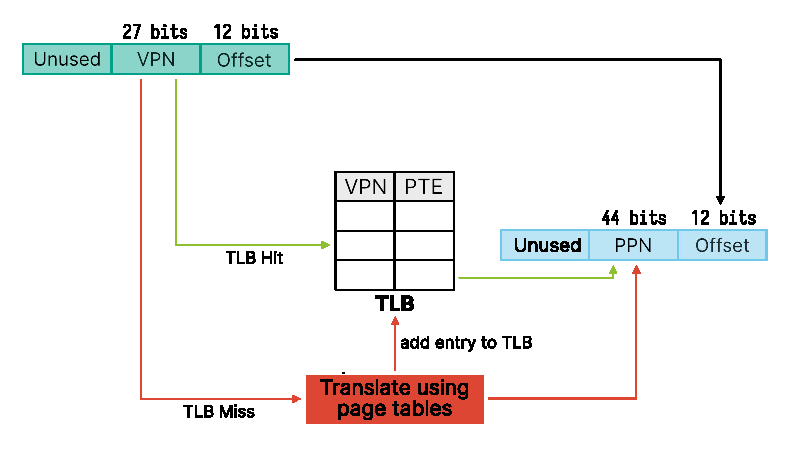
\includegraphics{tlb.eps}

\end{slide}

\begin{slide}

    \slidetitle{Effective Access Time (EAT)}

    Assume a single page table
    
    \leftspace{}(there's only one additional memory access in the page table)
    \medskip

    $\mathsf{TLB\_Hit\_Time = TLB\_Search + Mem}$

    $\mathsf{TLB\_Miss\_Time = TLB\_Search + 2 \times Mem}$

    $\mathsf{EAT = \alpha \times TLB\_Hit\_Time + (1 - \alpha) \times TLB\_Miss\_Time}$
    \medskip

    If $\mathsf{\alpha = 0.8}$, $\mathsf{TLB\_Search = 10\ ns}$, and accesses take 100 ns, calculate EAT

\end{slide}

\begin{slide}

    \slidetitle{Context Switches Require Handling the TLB}

    You can either flush the cache, or attach a process ID to the TLB
    \medskip

    Most implementation just flush the TLB

    \leftspace{}RISC-V uses a \texttt{sfence.vma} instruction to flush the TLB
    \medskip

    On x86 loading the base page table will also flush the TLB

\end{slide}

\begin{slide}
    
    \slidetitle{
      Computer Memory Hierarchy is a
    
      Trade-off of Capacity and Speed
    }

    \centering
    \begin{tikzpicture}[shorten >=0pt]
      \coordinate (A) at (-5,0) {};
      \coordinate (B) at ( 5,0) {};
      \coordinate (C) at (0,7) {};
      \draw[name path=AC] (A) -- (C);
      \draw[name path=BC] (B) -- (C);
      \foreach \y/\A in {
        0/Tape Drives,
        1/Hard Disk Drive (HDD),
        2/SATA Solid State Disk (SSD),
        3/Non-Volatile Memory (NVMe),
        4/Memory (RAM),
        5/CPU Cache,
        6/CPU
      } {
        \draw ($(A)!\y/7!(C)$) -- ($(B)!\y/7!(C)$)
          node[midway,above] {\A};
      }

      \draw [->, very thick] (-3,6) -- (-3,4) node[midway, left] {Capacity};
      \draw [->, very thick] (3,4) -- (3,6) node[midway, right] {Speed (and price)};
    \end{tikzpicture}

\end{slide}

\begin{slide}

    \slidetitle{We Want to Hide the Hierarchy from the User}

    Each level wants to pretend it has the speed of the layer above it

    \leftspace{}and the capacity of the layer below it
    \medskip

    The memory used by all the processes my exceed the amount of physical memory

    \leftspace{}Not all of them may be in use at the same time
    \medskip

    Only keep referenced pages in memory, put others on disk

    \leftspace{}Swap pages back to memory when they're needed

\end{slide}

\begin{slide}

    \slidetitle{Demand Paging}

    We use memory as a cache for the file system
    \medskip

    Map memory pages to file system blocks

    \leftspace{}Only load them into memory when they're used through
    the page fault handler
    \medskip

    If the page doesn't represent a file, we can map it to swap space

    \leftspace{}Move it to disk if we need to use more physical memory

\end{slide}

\begin{slide}

    \slidetitle{A Processes' Working Set Should Fit in Physical Memory}

    Given an amount of time, the number of pages your process uses
    is called
    its \textit{working set}
    \medskip

    If you cannot fit your working set into physical memory your process
    will \textit{thrash}

    \leftspace{}It's constantly moving entries in and out of cache

\end{slide}

\begin{slide}

    \slidetitle{Page Replacement Algorithms}

    Optimal

    \leftspace{}Replace the page that won't be used for the longest
    \medskip

    Random

    \leftspace{}Replace a random page
    \medskip

    First-in First-out (FIFO)

    \leftspace{}Replace the oldest page first
    \medskip

    Least Recently Used (LRU)

    \leftspace{}Replace the page that hasn't been used in the longest time

\end{slide}

\begin{slide}

    \slidetitle{Page Replacement Evaluation}

    Assume our physical memory can only hold 4 pages, and we access the following:

    \leftspace{}1 2 3 4 1 2 5 1 2 3 4 5 (all of the pages are initially on disk)
    \medskip

    We'll use this for a bunch of examples during this lecture

    \leftspace{}We want the fewest number of page faults
    \medskip

    For every example we'll find the number of page faults

\end{slide}

\begin{slide}

    \slidetitle{Optimal Example}

    Assume our physical memory can only hold 4 pages, and we access the following:

    \leftspace{}1 2 3 4 1 2 5 1 2 3 4 5 (all of the pages are initially on disk)

    \begin{center}
      \begin{tikzpicture}[
        every node/.style={
          align=center,
          text height=2ex,
          text width=1em
        },
        swapin/.list={
          (2,1),
          (3,2),
          (4,3),
          (5,4),
          (5,7),
          (2,11)
        },
      ]
        \matrix (m) [
          matrix of nodes,
          nodes in empty cells,
          column sep=1em,
          column 2/.style={visible on=<2->},
          column 3/.style={visible on=<3->},
          column 4/.style={visible on=<4->},
          column 5/.style={visible on=<5->},
          column 6/.style={visible on=<6->},
          column 7/.style={visible on=<7->},
          column 8/.style={visible on=<8->},
          column 9/.style={visible on=<9->},
          column 10/.style={visible on=<10->},
          column 11/.style={visible on=<11->},
          column 12/.style={visible on=<12->},
        ] {
          1 & 2 & 3 & 4 & 1 & 2 & 5 & 1 & 2 & 3 & 4 & 5 \\
          1 & 1 & 1 & 1 & 1 & 1 & 1 & 1 & 1 & 1 & 4 & 4 \\
            & 2 & 2 & 2 & 2 & 2 & 2 & 2 & 2 & 2 & 2 & 2 \\
            &   & 3 & 3 & 3 & 3 & 3 & 3 & 3 & 3 & 3 & 3 \\
            &   &   & 4 & 4 & 4 & 5 & 5 & 5 & 5 & 5 & 5 \\
        };
        \draw (m-2-1.north west) rectangle (m-5-1.south east);
        \draw (m-2-2.north west) rectangle (m-5-2.south east);
        \draw (m-2-3.north west) rectangle (m-5-3.south east);
        \draw (m-2-4.north west) rectangle (m-5-4.south east);
        \draw (m-2-5.north west) rectangle (m-5-5.south east);
        \draw (m-2-6.north west) rectangle (m-5-6.south east);
        \draw (m-2-7.north west) rectangle (m-5-7.south east);
        \draw (m-2-8.north west) rectangle (m-5-8.south east);
        \draw (m-2-9.north west) rectangle (m-5-9.south east);
        \draw (m-2-10.north west) rectangle (m-5-10.south east);
        \draw (m-2-11.north west) rectangle (m-5-11.south east);
        \draw (m-2-12.north west) rectangle (m-5-12.south east);
      \end{tikzpicture}
    \end{center}

    \begin{flushright}
      \onslide<13->{6 page faults}
    \end{flushright}

\end{slide}

\begin{slide}

    \slidetitle{FIFO Example}

    Assume our physical memory can only hold 4 pages, and we access the following:

    \leftspace{}1 2 3 4 1 2 5 1 2 3 4 5 (all of the pages are initially on disk)

    \begin{center}
      \begin{tikzpicture}[
        every node/.style={
          align=center,
          text height=2ex,
          text width=1em
        },
        swapin/.list={
          (2,1),
          (3,2),
          (4,3),
          (5,4),
          (2,7),
          (3,8),
          (4,9),
          (5,10),
          (2,11),
          (3,12)
        },
      ]
        \matrix (m) [
          matrix of nodes,
          nodes in empty cells,
          column sep=1em,
          column 2/.style={visible on=<2->},
          column 3/.style={visible on=<3->},
          column 4/.style={visible on=<4->},
          column 5/.style={visible on=<5->},
          column 6/.style={visible on=<6->},
          column 7/.style={visible on=<7->},
          column 8/.style={visible on=<8->},
          column 9/.style={visible on=<9->},
          column 10/.style={visible on=<10->},
          column 11/.style={visible on=<11->},
          column 12/.style={visible on=<12->},
        ] {
          1 & 2 & 3 & 4 & 1 & 2 & 5 & 1 & 2 & 3 & 4 & 5 \\
          1 & 1 & 1 & 1 & 1 & 1 & 5 & 5 & 5 & 5 & 4 & 4 \\
            & 2 & 2 & 2 & 2 & 2 & 2 & 1 & 1 & 1 & 1 & 5 \\
            &   & 3 & 3 & 3 & 3 & 3 & 3 & 2 & 2 & 2 & 2 \\
            &   &   & 4 & 4 & 4 & 4 & 4 & 4 & 3 & 3 & 3 \\
        };
        \draw (m-2-1.north west) rectangle (m-5-1.south east);
        \draw (m-2-2.north west) rectangle (m-5-2.south east);
        \draw (m-2-3.north west) rectangle (m-5-3.south east);
        \draw (m-2-4.north west) rectangle (m-5-4.south east);
        \draw (m-2-5.north west) rectangle (m-5-5.south east);
        \draw (m-2-6.north west) rectangle (m-5-6.south east);
        \draw (m-2-7.north west) rectangle (m-5-7.south east);
        \draw (m-2-8.north west) rectangle (m-5-8.south east);
        \draw (m-2-9.north west) rectangle (m-5-9.south east);
        \draw (m-2-10.north west) rectangle (m-5-10.south east);
        \draw (m-2-11.north west) rectangle (m-5-11.south east);
        \draw (m-2-12.north west) rectangle (m-5-12.south east);
      \end{tikzpicture}
    \end{center}

    \begin{flushright}
      \onslide<13->{10 page faults}
    \end{flushright}

\end{slide}

\begin{slide}

    \slidetitle{FIFO Example (3 Page Frames)}

    Assume our physical memory can only hold \textbf{3} pages, and we access the following:

    \leftspace{}1 2 3 4 1 2 5 1 2 3 4 5 (all of the pages are initially on disk)

    \begin{center}
      \begin{tikzpicture}[
        every node/.style={
          align=center,
          text height=2ex,
          text width=1em
        },
        swapin/.list={
          (2,1),
          (3,2),
          (4,3),
          (2,4),
          (3,5),
          (4,6),
          (2,7),
          (3,10),
          (4,11)
        },
      ]
        \matrix (m) [
          matrix of nodes,
          nodes in empty cells,
          column sep=1em,
          column 2/.style={visible on=<2->},
          column 3/.style={visible on=<3->},
          column 4/.style={visible on=<4->},
          column 5/.style={visible on=<5->},
          column 6/.style={visible on=<6->},
          column 7/.style={visible on=<7->},
          column 8/.style={visible on=<8->},
          column 9/.style={visible on=<9->},
          column 10/.style={visible on=<10->},
          column 11/.style={visible on=<11->},
          column 12/.style={visible on=<12->},
        ] {
          1 & 2 & 3 & 4 & 1 & 2 & 5 & 1 & 2 & 3 & 4 & 5 \\
          1 & 1 & 1 & 4 & 4 & 4 & 5 & 5 & 5 & 5 & 5 & 5 \\
            & 2 & 2 & 2 & 1 & 1 & 1 & 1 & 1 & 3 & 3 & 3 \\
            &   & 3 & 3 & 3 & 2 & 2 & 2 & 2 & 2 & 4 & 4 \\
        };
        \draw (m-2-1.north west) rectangle (m-4-1.south east);
        \draw (m-2-2.north west) rectangle (m-4-2.south east);
        \draw (m-2-3.north west) rectangle (m-4-3.south east);
        \draw (m-2-4.north west) rectangle (m-4-4.south east);
        \draw (m-2-5.north west) rectangle (m-4-5.south east);
        \draw (m-2-6.north west) rectangle (m-4-6.south east);
        \draw (m-2-7.north west) rectangle (m-4-7.south east);
        \draw (m-2-8.north west) rectangle (m-4-8.south east);
        \draw (m-2-9.north west) rectangle (m-4-9.south east);
        \draw (m-2-10.north west) rectangle (m-4-10.south east);
        \draw (m-2-11.north west) rectangle (m-4-11.south east);
        \draw (m-2-12.north west) rectangle (m-4-12.south east);
      \end{tikzpicture}
    \end{center}

    \begin{flushright}
      \onslide<13->{9 page faults}
    \end{flushright}

\end{slide}

\begin{slide}

    \slidetitle{Bélády's Anomaly Says More Page Frames Causes More Faults}

    This is a problem with FIFO algorithms

    \leftspace{}Does not exist with LRU or ``stack-based algorithms''
    \medskip

    Paper in 2010 found that this FIFO anomaly is unbounded (\url{https://arxiv.org/abs/1003.1336})

    \leftspace{}You could construct a sequence to get any arbitrary page fault ratio
    \medskip

    For other algorithms:

    \leftspace{}increasing the number of page frames decreases the number of
    page faults

\end{slide}

\begin{slide}

    \slidetitle{LRU Example (Use FIFO to Break Ties)}

    Assume our physical memory can only hold 4 pages, and we access the following:

    \leftspace{}1 2 3 4 1 2 5 1 2 3 4 5 (all of the pages are initially on disk)

    \begin{center}
      \begin{tikzpicture}[
        every node/.style={
          align=center,
          text height=2ex,
          text width=1em
        },
        swapin/.list={
          (2,1),
          (3,2),
          (4,3),
          (5,4),
          (4,7),
          (5,10),
          (4,11),
          (2,12)
        },
      ]
        \matrix (m) [
          matrix of nodes,
          nodes in empty cells,
          column sep=1em,
          column 2/.style={visible on=<2->},
          column 3/.style={visible on=<3->},
          column 4/.style={visible on=<4->},
          column 5/.style={visible on=<5->},
          column 6/.style={visible on=<6->},
          column 7/.style={visible on=<7->},
          column 8/.style={visible on=<8->},
          column 9/.style={visible on=<9->},
          column 10/.style={visible on=<10->},
          column 11/.style={visible on=<11->},
          column 12/.style={visible on=<12->},
        ] {
          1 & 2 & 3 & 4 & 1 & 2 & 5 & 1 & 2 & 3 & 4 & 5 \\
          1 & 1 & 1 & 1 & 1 & 1 & 1 & 1 & 1 & 1 & 1 & 5 \\
            & 2 & 2 & 2 & 2 & 2 & 2 & 2 & 2 & 2 & 2 & 2 \\
            &   & 3 & 3 & 3 & 3 & 5 & 5 & 5 & 5 & 4 & 4 \\
            &   &   & 4 & 4 & 4 & 4 & 4 & 4 & 3 & 3 & 3 \\
        };
        \draw (m-2-1.north west) rectangle (m-5-1.south east);
        \draw (m-2-2.north west) rectangle (m-5-2.south east);
        \draw (m-2-3.north west) rectangle (m-5-3.south east);
        \draw (m-2-4.north west) rectangle (m-5-4.south east);
        \draw (m-2-5.north west) rectangle (m-5-5.south east);
        \draw (m-2-6.north west) rectangle (m-5-6.south east);
        \draw (m-2-7.north west) rectangle (m-5-7.south east);
        \draw (m-2-8.north west) rectangle (m-5-8.south east);
        \draw (m-2-9.north west) rectangle (m-5-9.south east);
        \draw (m-2-10.north west) rectangle (m-5-10.south east);
        \draw (m-2-11.north west) rectangle (m-5-11.south east);
        \draw (m-2-12.north west) rectangle (m-5-12.south east);
      \end{tikzpicture}
    \end{center}

    \begin{flushright}
      \onslide<13->{8 page faults}
    \end{flushright}

\end{slide}

\begin{slide}

    \slidetitle{Implementing LRU in Hardware Has to Search All Pages}

    You could implement it by keeping a counter for each page
    \medskip

    For each page reference, save the system clock into the counter
    \medskip


    For replacement, scan through the pages and find the one with the oldest clock

\end{slide}

\begin{slide}

    \slidetitle{Implementing LRU in Software is Too Expensive}

    Create a doubly linked list of pages
    \medskip

    For each page reference, move it to the front of the list
    \medskip

    For replacement, remove from the back of the list
    \medskip

    It requires 6 pointer updates for each page reference, and

    \leftspace{}also creates a high contention bottleneck for multiple processors

\end{slide}

\begin{slide}

    \slidetitle{Implementing LRU in Practice Isn't Going to Work}

    We settle for approximate LRU

    \leftspace{}LRU is an approximation of the optimal case anyways
    \medskip

    There's lots of different tweaks you can do to implement it more efficiently
    \medskip

    We'll be looking at the clock algorithm, but there's also:

    \leftspace{}Least Frequently Used (LFU), 2Q, Adaptive Replacement Cache (ARC)

\end{slide}

\begin{slide}

    \slidetitle{Page Replacement Algorithms Aim to Reduce Page Faults}

    We saw the following:
    \begin{itemize}
      \item Optimal (good for comparison but not realistic)
      \item Random (actually works surprisingly well, avoids the worst case)
      \item FIFO (easy to implement but Bélády's anomaly)
      \item LRU (gets close to optimal but expensive to implement)
    \end{itemize}

\end{slide}


\begin{slide}

	\slidetitle{Paging Revisit}
	
	\vspace{-5mm}
	
	\begin{itemize}
		\item \texttt{int A[100];}
		\item All instructions are on page 0.
		\item Each page holds 64 entries (64 integers). 
		\item Array A starts at location 64. 
	\end{itemize}
	
\end{slide}

\begin{slide}

	\slidetitle{Page Replacement Algorithm}
	
	Memory can hold only a limited number of pages.
	
	\medskip

	When memory is full, a page must be swapped out to swap space (where?).
	
	\medskip
	
	The OS decides which page to replace using a Page Replacement Algorithm.

	\medskip
	
	Goal: Keep the most useful pages in memory to improve performance (reduce the number of page faults).

\end{slide}

\begin{slide}

    \slidetitle{Optimal Example}

    Assume our physical memory can only hold 4 pages, and we access the following:

    \leftspace{}1 2 3 4 1 2 5 1 2 3 4 5 (all of the pages are initially on disk)

    \begin{center}
      \begin{tikzpicture}[
        every node/.style={
          align=center,
          text height=2ex,
          text width=1em
        }
      ]
        \matrix (m) [
          matrix of nodes,
          nodes in empty cells,
          column sep=1em
        ] {
          1 & 2 & 3 & 4 & 1 & 2 & 5 & 1 & 2 & 3 & 4 & 5 \\
          1 & 1 & 1 & 1 & 1 & 1 & 1 & 1 & 1 & 1 & 4 & 4 \\
            & 2 & 2 & 2 & 2 & 2 & 2 & 2 & 2 & 2 & 2 & 2 \\
            &   & 3 & 3 & 3 & 3 & 3 & 3 & 3 & 3 & 3 & 3 \\
            &   &   & 4 & 4 & 4 & 5 & 5 & 5 & 5 & 5 & 5 \\
        };
        \foreach \x in {1,...,12} {
          \draw (m-2-\x.north west) rectangle (m-5-\x.south east);
        }
      \end{tikzpicture}
    \end{center}

    \begin{flushright}
      6 page faults
    \end{flushright}

\end{slide}

\begin{slide}

    \slidetitle{FIFO Example}

    Assume our physical memory can only hold 4 pages, and we access the following:

    \leftspace{}1 2 3 4 1 2 5 1 2 3 4 5 (all of the pages are initially on disk)

    \begin{center}
      \begin{tikzpicture}[
        every node/.style={
          align=center,
          text height=2ex,
          text width=1em
        },
        swapin/.list={
          (2,1),
          (3,2),
          (4,3),
          (5,4),
          (2,7),
          (3,8),
          (4,9),
          (5,10),
          (2,11),
          (3,12)
        },
      ]
        \matrix (m) [
          matrix of nodes,
          nodes in empty cells,
          column sep=1em,
          column 2/.style={visible on=<2->},
          column 3/.style={visible on=<3->},
          column 4/.style={visible on=<4->},
          column 5/.style={visible on=<5->},
          column 6/.style={visible on=<6->},
          column 7/.style={visible on=<7->},
          column 8/.style={visible on=<8->},
          column 9/.style={visible on=<9->},
          column 10/.style={visible on=<10->},
          column 11/.style={visible on=<11->},
          column 12/.style={visible on=<12->},
        ] {
          1 & 2 & 3 & 4 & 1 & 2 & 5 & 1 & 2 & 3 & 4 & 5 \\
          1 & 1 & 1 & 1 & 1 & 1 & 5 & 5 & 5 & 5 & 4 & 4 \\
            & 2 & 2 & 2 & 2 & 2 & 2 & 1 & 1 & 1 & 1 & 5 \\
            &   & 3 & 3 & 3 & 3 & 3 & 3 & 2 & 2 & 2 & 2 \\
            &   &   & 4 & 4 & 4 & 4 & 4 & 4 & 3 & 3 & 3 \\
        };
        \draw (m-2-1.north west) rectangle (m-5-1.south east);
        \draw (m-2-2.north west) rectangle (m-5-2.south east);
        \draw (m-2-3.north west) rectangle (m-5-3.south east);
        \draw (m-2-4.north west) rectangle (m-5-4.south east);
        \draw (m-2-5.north west) rectangle (m-5-5.south east);
        \draw (m-2-6.north west) rectangle (m-5-6.south east);
        \draw (m-2-7.north west) rectangle (m-5-7.south east);
        \draw (m-2-8.north west) rectangle (m-5-8.south east);
        \draw (m-2-9.north west) rectangle (m-5-9.south east);
        \draw (m-2-10.north west) rectangle (m-5-10.south east);
        \draw (m-2-11.north west) rectangle (m-5-11.south east);
        \draw (m-2-12.north west) rectangle (m-5-12.south east);
      \end{tikzpicture}
    \end{center}

    \begin{flushright}
      \onslide<13->{10 page faults}
    \end{flushright}

\end{slide}

\begin{slide}

    \slidetitle{LRU Example (Use FIFO to Break Ties)}

    Assume our physical memory can only hold 4 pages, and we access the following:

    \leftspace{}1 2 3 4 1 2 5 1 2 3 4 5 (all of the pages are initially on disk)

    \begin{center}
      \begin{tikzpicture}[
        every node/.style={
          align=center,
          text height=2ex,
          text width=1em
        },
        swapin/.list={
          (2,1),
          (3,2),
          (4,3),
          (5,4),
          (4,7),
          (5,10),
          (4,11),
          (2,12)
        },
      ]
        \matrix (m) [
          matrix of nodes,
          nodes in empty cells,
          column sep=1em,
          column 2/.style={visible on=<2->},
          column 3/.style={visible on=<3->},
          column 4/.style={visible on=<4->},
          column 5/.style={visible on=<5->},
          column 6/.style={visible on=<6->},
          column 7/.style={visible on=<7->},
          column 8/.style={visible on=<8->},
          column 9/.style={visible on=<9->},
          column 10/.style={visible on=<10->},
          column 11/.style={visible on=<11->},
          column 12/.style={visible on=<12->},
        ] {
          1 & 2 & 3 & 4 & 1 & 2 & 5 & 1 & 2 & 3 & 4 & 5 \\
          1 & 1 & 1 & 1 & 1 & 1 & 1 & 1 & 1 & 1 & 1 & 5 \\
            & 2 & 2 & 2 & 2 & 2 & 2 & 2 & 2 & 2 & 2 & 2 \\
            &   & 3 & 3 & 3 & 3 & 5 & 5 & 5 & 5 & 4 & 4 \\
            &   &   & 4 & 4 & 4 & 4 & 4 & 4 & 3 & 3 & 3 \\
        };
        \draw (m-2-1.north west) rectangle (m-5-1.south east);
        \draw (m-2-2.north west) rectangle (m-5-2.south east);
        \draw (m-2-3.north west) rectangle (m-5-3.south east);
        \draw (m-2-4.north west) rectangle (m-5-4.south east);
        \draw (m-2-5.north west) rectangle (m-5-5.south east);
        \draw (m-2-6.north west) rectangle (m-5-6.south east);
        \draw (m-2-7.north west) rectangle (m-5-7.south east);
        \draw (m-2-8.north west) rectangle (m-5-8.south east);
        \draw (m-2-9.north west) rectangle (m-5-9.south east);
        \draw (m-2-10.north west) rectangle (m-5-10.south east);
        \draw (m-2-11.north west) rectangle (m-5-11.south east);
        \draw (m-2-12.north west) rectangle (m-5-12.south east);
      \end{tikzpicture}
    \end{center}

    \begin{flushright}
      \onslide<13->{8 page faults}
    \end{flushright}

\end{slide}

\begin{slide}

    \slidetitle{Implementing LRU in Practice Isn't Going to Work}

    We settle for approximate LRU

    \leftspace{}LRU is an approximation of the optimal case anyways
    \medskip

    There's lots of different tweaks you can do to implement it more efficiently
    \medskip

    We'll be looking at the clock algorithm, but there's also:

    \leftspace{}Least Frequently Used (LFU), 2Q, Adaptive Replacement Cache (ARC)

\end{slide}

\begin{slide}

    \slidetitle{Clock Algorithm}

    Data structures:
    \begin{itemize}
      \item Keeps a circular list of pages in memory
      \item Uses a reference bit for each page in memory (light grey in next slides)
      \item Has a ``hand'' (iterator) pointing to the last element examined
    \end{itemize}
    \medskip

    Algorithm, to insert a new page:
    \begin{itemize}
      \item Check the hand's reference bit, if it's 0 then place the page and advance hand
      \item If the reference bit is 1, set it to 0, advance the hand, and repeat
    \end{itemize}
    \medskip

    For page accesses, set the reference bit to 1

\end{slide}

\begin{slide}

    \slidetitle{Clock Example (with Diagram)}

	\vspace{-5mm}
	
    Assume our physical memory can only hold 4 pages, and we access the following:

    \leftspace{}1 2 3 4 5 2 3 1 2 3 (all of the pages are initially on disk)

	\vspace{-2mm}
	
    \begin{center}
      \begin{tikzpicture}
        \matrix (m) [
          matrix of nodes,
          nodes in empty cells,
          minimum width=2em,
          minimum height=2em,
          align=center,
          column sep=1em,
          column 1/.style={visible on=<2->},
          column 2/.style={visible on=<3->},
          column 3/.style={visible on=<4->},
          column 4/.style={visible on=<5->},
          column 5/.style={visible on=<6->},
          column 6/.style={visible on=<11->},
          column 7/.style={visible on=<12->},
          column 8/.style={visible on=<13->},
          column 9/.style={visible on=<16->},
          column 10/.style={visible on=<17->},
        ] {
          1 & 2 & 3 & 4 & 5 & 2 & 3 & 1 & 2 & 3 \\
        };
      \end{tikzpicture}

      \begin{tikzpicture}[
        box/.style={
          draw,
          align=center,
          minimum width=2em,
          minimum height=6em,
          rectangle split,
          rectangle split parts=2,
          rectangle split part fill={white, black!20},
        }
      ]

        \node (c) at (0, 0) {};

        \node<1> [above=of c, box] (n) {0 \nodepart{second} 0};
        \node<2-5> [above=of c, box] {1 \nodepart{second} 1};
        \node<6-9> [above=of c, box] {1 \nodepart{second} 0};
        \node<10-> [above=of c, box] {5 \nodepart{second} 1};

        \node<1-2> [right=of c, box] (e) {0 \nodepart{second} 0};
        \node<3-6,11-12,16-> [right=of c, box] {2 \nodepart{second} 1};
        \node<7-10,13-15> [right=of c, box] {2 \nodepart{second} 0};

        \node<1-3> [below=of c, box] (s) {0 \nodepart{second} 0};
        \node<4-7,12-13,17-> [below=of c, box] {3 \nodepart{second} 1};
        \node<8-11,14-16> [below=of c, box] {3 \nodepart{second} 0};

        \node<1-4> [left=of c, box] (w) {0 \nodepart{second} 0};
        \node<5-8> [left=of c, box] (w) {4 \nodepart{second} 1};
        \node<9-14> [left=of c, box] (w) {4 \nodepart{second} 0};
        \node<15-> [left=of c, box] (w) {1 \nodepart{second} 1};

        \path [->] (n) edge [bend left] (e)
                   (e) edge [bend left] (s)
                   (s) edge [bend left] (w)
                   (w) edge [bend left] (n);

        \path<1,5,9,15-> [->] (c) edge (n);
        \path<2,6,10-12> [->] (c) edge (e);
        \path<3,7,13> [->] (c) edge (s);
        \path<4,8,14> [->] (c) edge (w);

      \end{tikzpicture}
    \end{center}

\end{slide}

\begin{slide}

    \slidetitle{Clock Example}

    Assume our physical memory can only hold 4 pages, and we access the following:

    \leftspace{}1 2 3 4 5 2 3 1 2 3 (all of the pages are initially on disk)

    \begin{center}
      \begin{tikzpicture}[
        every node/.style={
          align=center,
          text height=2ex,
          text width=1em
        }
      ]
        \matrix (m) [
          matrix of nodes,
          nodes in empty cells,
          column sep=1em
        ] {
          1 & 2 & 3 & 4 & 5 & 2 & 3 & 1 & 2 & 3 \\
          1 & 1 & 1 & 1 & 5 & 5 & 5 & 5 & 5 & 5 \\
            & 2 & 2 & 2 & 2 & 2 & 2 & 2 & 2 & 2 \\
            &   & 3 & 3 & 3 & 3 & 3 & 3 & 3 & 3 \\
            &   &   & 4 & 4 & 4 & 4 & 1 & 1 & 1 \\
        };
        \foreach \x in {1,...,10} {
          \draw (m-2-\x.north west) rectangle (m-5-\x.south east);
        }
      \end{tikzpicture}
    \end{center}

    \begin{flushright}
      6 page faults
    \end{flushright}

\end{slide}

\begin{slide}

    \slidetitle{The Buddy Allocator Restricts the Problem}

    Typically, allocation requests are of size $\mathsf{2^n}$

    \leftspace{}e.g. 2, 4, 8, 16, 32, ..., 4096, ...
    \medskip

    Restrict allocations to be powers of 2 to enable a more efficient
    implementation

    \leftspace{}Split blocks into 2 until you can handle the request
    \medskip

    We want to be able to do fast searching and merging

  \end{slide}

  \begin{slide}

    \slidetitle{You Can Implement the Buddy Allocator Using Multiple Lists}

    We restrict the requests to be $\mathsf{2^k, 0 \leq k \leq N}$ (round up if
    needed)
    \medskip

    Our implementation would use $\mathsf{N+1}$ free lists of blocks for each
    size
    \medskip

    For a request of size $\mathsf{2^k}$, search the free list until we find
    a big enough block

    \leftspace{}Search $\mathsf{k, k+1, k+2, ...}$ until we find one

    \leftspace{}\leftspace{}Recursively divide the block if needed until it's
    the correct size

    \leftspace{}\leftspace{}Insert “buddy” blocks into free lists
    \medskip

    For deallocations, we coalesce the buddy blocks back together

    \leftspace{}Recursively coalesce the blocks if needed

  \end{slide}

  \begin{slide}
    
    \slidetitle{Using the Buddy Allocator (1)}

    \begin{tikzpicture}[node distance=5mm and 0mm]
            
        \node[draw,rectangle,minimum width=280,minimum height=20,fill=black,text=white]    (a00)        {256};
        \node[draw,rectangle,minimum width=140,minimum height=20,fill=black,text=white,xshift=-70]    (a10) [below=of a00]       {128};
        \node[draw,rectangle,minimum width=140,minimum height=20,fill=black,text=white]    (a11) [right=of a10]       {128};
        \node[draw,rectangle,minimum width=70,minimum height=20,fill=black,text=white,xshift=-35]    (a20) [below=of a10]       {64};
        \node[draw,rectangle,minimum width=70,minimum height=20]    (a21) [right=of a20]       {64};
        \node[draw,rectangle,minimum width=70,minimum height=20,fill=pantone633,xshift=-35]    (a22) [below=of a11]       {64};
        \node[draw,rectangle,minimum width=70,minimum height=20]    (a23) [right=of a22]       {64};
        \node[draw,rectangle,minimum width=35,minimum height=20,fill=pantonewarmred,xshift=-17]    (a30) [below=of a20]       {32};
        \node[draw,rectangle,minimum width=35,minimum height=20]    (a31) [right=of a30]       {32};

        \draw[->] (a00.south) -- (a10.north);
        \draw[->] (a00.south) -- (a11.north);
        \draw[->] (a10.south) -- (a20.north);
        \draw[->] (a10.south) -- (a21.north);
        \draw[->] (a11.south) -- (a22.north);
        \draw[->] (a11.south) -- (a23.north);
        \draw[->] (a20.south) -- (a30.north);
        \draw[->] (a20.south) -- (a31.north);

    \end{tikzpicture}
    \medskip

    Where do we allocate a request of size 28?

  \end{slide}

  \begin{slide}
    
    \slidetitle{Using the Buddy Allocator (2)}

    \begin{tikzpicture}[node distance=5mm and 0mm]
            
        \node[draw,rectangle,minimum width=280,minimum height=20,fill=black,text=white]    (a00)        {256};
        \node[draw,rectangle,minimum width=140,minimum height=20,fill=black,text=white,xshift=-70]    (a10) [below=of a00]       {128};
        \node[draw,rectangle,minimum width=140,minimum height=20,fill=black,text=white]    (a11) [right=of a10]       {128};
        \node[draw,rectangle,minimum width=70,minimum height=20,fill=black,text=white,xshift=-35]    (a20) [below=of a10]       {64};
        \node[draw,rectangle,minimum width=70,minimum height=20]    (a21) [right=of a20]       {64};
        \node[draw,rectangle,minimum width=70,minimum height=20,fill=pantone633,xshift=-35]    (a22) [below=of a11]       {64};
        \node[draw,rectangle,minimum width=70,minimum height=20]    (a23) [right=of a22]       {64};
        \node[draw,rectangle,minimum width=35,minimum height=20,fill=pantonewarmred,xshift=-17]    (a30) [below=of a20]       {32};
        \node[draw,rectangle,minimum width=35,minimum height=20,fill=pantone376]    (a31) [right=of a30]       {32};

        \draw[->] (a00.south) -- (a10.north);
        \draw[->] (a00.south) -- (a11.north);
        \draw[->] (a10.south) -- (a20.north);
        \draw[->] (a10.south) -- (a21.north);
        \draw[->] (a11.south) -- (a22.north);
        \draw[->] (a11.south) -- (a23.north);
        \draw[->] (a20.south) -- (a30.north);
        \draw[->] (a20.south) -- (a31.north);

    \end{tikzpicture}
    \medskip

    Where do we allocate a request of size 32?

  \end{slide}

  \begin{slide}
    
    \slidetitle{Using the Buddy Allocator (3)}

    \begin{tikzpicture}[node distance=5mm and 0mm]
            
        \node[draw,rectangle,minimum width=280,minimum height=20,fill=black,text=white]    (a00)        {256};
        \node[draw,rectangle,minimum width=140,minimum height=20,fill=black,text=white,xshift=-70]    (a10) [below=of a00]       {128};
        \node[draw,rectangle,minimum width=140,minimum height=20,fill=black,text=white]    (a11) [right=of a10]       {128};
        \node[draw,rectangle,minimum width=70,minimum height=20,fill=black,text=white,xshift=-35]    (a20) [below=of a10]       {64};
        \node[draw,rectangle,minimum width=70,minimum height=20,fill=black,text=white]    (a21) [right=of a20]       {64};
        \node[draw,rectangle,minimum width=70,minimum height=20,fill=pantone633,xshift=-35]    (a22) [below=of a11]       {64};
        \node[draw,rectangle,minimum width=70,minimum height=20]    (a23) [right=of a22]       {64};
        \node[draw,rectangle,minimum width=35,minimum height=20,fill=pantonewarmred,xshift=-17]    (a30) [below=of a20]       {32};
        \node[draw,rectangle,minimum width=35,minimum height=20,fill=pantone376]    (a31) [right=of a30]  {32};
        \node[draw,rectangle,minimum width=35,minimum height=20,fill=pantone2613!50,xshift=-17]    (a32) [below=of a21]       {32};
        \node[draw,rectangle,minimum width=35,minimum height=20,]    (a33) [right=of a32]       {32};

        \draw[->] (a00.south) -- (a10.north);
        \draw[->] (a00.south) -- (a11.north);
        \draw[->] (a10.south) -- (a20.north);
        \draw[->] (a10.south) -- (a21.north);
        \draw[->] (a11.south) -- (a22.north);
        \draw[->] (a11.south) -- (a23.north);
        \draw[->] (a20.south) -- (a30.north);
        \draw[->] (a20.south) -- (a31.north);
        \draw[->] (a21.south) -- (a32.north);
        \draw[->] (a21.south) -- (a33.north);

    \end{tikzpicture}
    \medskip

    What happens when we free the size 64 block?

\end{slide}

\begin{slide}
  
  \slidetitle{Using the Buddy Allocator (4)}

  \begin{tikzpicture}[node distance=5mm and 0mm]
          
      \node[draw,rectangle,minimum width=280,minimum height=20,fill=black,text=white]    (a00)        {256};
      \node[draw,rectangle,minimum width=140,minimum height=20,fill=black,text=white,xshift=-70]    (a10) [below=of a00]       {128};
      \node[draw,rectangle,minimum width=140,minimum height=20]    (a11) [right=of a10]       {128};
      \node[draw,rectangle,minimum width=70,minimum height=20,fill=black,text=white,xshift=-35]    (a20) [below=of a10]       {64};
      \node[draw,rectangle,minimum width=70,minimum height=20,fill=black,text=white]    (a21) [right=of a20]       {64};
      \node[draw,rectangle,minimum width=35,minimum height=20,fill=pantonewarmred,xshift=-17]    (a30) [below=of a20]       {32};
      \node[draw,rectangle,minimum width=35,minimum height=20,fill=pantone376]    (a31) [right=of a30]  {32};
      \node[draw,rectangle,minimum width=35,minimum height=20,fill=pantone2613!50,xshift=-17]    (a32) [below=of a21]       {32};
      \node[draw,rectangle,minimum width=35,minimum height=20,]    (a33) [right=of a32]       {32};

      \draw[->] (a00.south) -- (a10.north);
      \draw[->] (a00.south) -- (a11.north);
      \draw[->] (a10.south) -- (a20.north);
      \draw[->] (a10.south) -- (a21.north);
      \draw[->] (a20.south) -- (a30.north);
      \draw[->] (a20.south) -- (a31.north);
      \draw[->] (a21.south) -- (a32.north);
      \draw[->] (a21.south) -- (a33.north);

  \end{tikzpicture}

\end{slide}

\begin{slide}

  \slidetitle{Buddy Allocators are Used in Linux}

  Advantages

  \leftspace{}Fast and simple compared to general dynamic memory allocation

  \leftspace{}Avoids external fragmentation by keeping free physical pages contiguous
  \medskip

  Disadvantages

  \leftspace{}There's always internal fragmentation

  \leftspace{}\leftspace{}We always round up the allocation size if it's not a
  power of 2

\end{slide}

\begin{slide}
  
  \slidetitle{Slab Allocators Take Advantage of Fixed Size Allocations}

  Allocate objects of same size from a dedicated pool

  \leftspace{}All structures of the same type are the same size
  \medskip

  Every object type has it's own pool with blocks of the correct size

  \leftspace{}This prevents internal fragmentation

\end{slide}

\begin{slide}

  \slidetitle{Slab is a Cache of ``Slots''}

  Each allocation size has a corresponding slab of slots
  
  (one slot holds one allocation)
  \medskip

  Instead of a linked list, we can use a bitmap
  
  (there's a mapping between bit and slot)

  \leftspace{}For allocations, we set the bit and return the slot

  \leftspace{}For deallocations, we just clear the bit
  \medskip

  The slab can be implemented on top of the buddy allocator

\end{slide}

\begin{slide}
  
  \slidetitle{Each Slab Can Be Allocated using the Buddy Allocator}
  
  Consider two object sizes: A and B
  \medskip
  
  \begin{tikzpicture}[node distance=0mm and 0mm]

      \node[draw,rectangle,minimum width=20,minimum height=20,fill=pantonewarmred]    (a0)        {};
      \node[draw,rectangle,minimum width=20,minimum height=20]    (a1)     [right=of a0]   {};
      \node[draw,rectangle,minimum width=20,minimum height=20]    (a2)     [right=of a1]   {};
      \node[draw,rectangle,minimum width=20,minimum height=20,fill=pantonewarmred]    (a3)     [right=of a2]   {};
      \node[draw,rectangle,minimum width=8,minimum height=20,fill=black]    (a4)     [right=of a3]   {};

      \node[draw,rectangle,minimum width=20,minimum height=20]    (a5)     [right=of a4]   {};
      \node[draw,rectangle,minimum width=20,minimum height=20]    (a6)     [right=of a5]   {};
      \node[draw,rectangle,minimum width=20,minimum height=20]    (a7)     [right=of a6]   {};
      \node[draw,rectangle,minimum width=20,minimum height=20]    (a8)     [right=of a7]   {};
      \node[draw,rectangle,minimum width=8,minimum height=20,fill=black]    (a9)     [right=of a8]   {};


      \node[draw,rectangle,minimum width=40,minimum height=20,fill=pantonewarmred]    (b1)     [right=of a9]   {};
      \node[draw,rectangle,minimum width=40,minimum height=20,fill=pantonewarmred]    (b2)     [right=of b1]   {};

      \node[draw,rectangle,minimum width=40,minimum height=20]    (b3)     [right=of b2]   {};
      \node[draw,rectangle,minimum width=40,minimum height=20]    (b4)     [right=of b3]   {};

      \node[draw,rectangle,minimum width=90,minimum height=20,xshift=35]    (s0)    [below=of a0]   {Slab A1};
      \node[draw,rectangle,minimum width=90,minimum height=20]    (s1)    [right=of s0]   {Slab A2};
      \node[draw,rectangle,minimum width=80,minimum height=20]    (s2)    [right=of s1]   {Slab B1};
      \node[draw,rectangle,minimum width=80,minimum height=20]    (s3)    [right=of s2]   {Slab B2};

  \end{tikzpicture}
  \medskip

  We can reduce internal fragmentation if Slabs are located
  adjacently

  \leftspace{}In this example A has internal fragmentation (dark box)

\end{slide}

\begin{slide}
  
  \slidetitle{Journaling Filesystem}

  Deleting a file on a Unix file system involves three steps:

  \begin{enumerate}
    \item Removing its directory entry.
    \item Releasing the inode to the pool of free inodes.
    \item Returning all disk blocks to the pool of free disk blocks.
  \end{enumerate}
  \medskip

  Crashes could occur between any steps, leading to a storage leak
  \medskip

  The journal contains operations in progress, so if a crash occurs we can
  recover

\end{slide}


\end{document}
